\graphicspath{{images/}}

\section*{Komplexitätstheorie}

\begin{definition}{Quantitative Gesetze und Grenzen}
    der algorithmischen Informationsverarbeitung

    \begin{itemize}
    \item Zeitkomplexität: Laufzeit des besten Programms, welches das Problem löst
    \item Platzkomplexität: Speicherplatz des besten Programms
    \item Beschreibungskomplexität: Länge des kürzesten Programms
    \end{itemize}
\end{definition}

\begin{theorem}{Zeitbedarf}
    Der Zeitbedarf von $M$ auf Eingaben der Länge $n \in \mathbb{N}$ im schlechtesten Fall definiert als
    $$
    \operatorname{Time}_{M}(n)=\max \left\{\operatorname{Time}_{M}(\omega)|| \omega \mid=n\right\}
    $$
    Sei $M$ eine TM, die immer hält und sei $\omega \in \Sigma^{*}$. Der Zeitbedarf von $M$ auf der Eingabe $\omega$ ist
    \begin{itemize}
    \item Time $_{M}(\omega)=$ Anzahl von Konfigurationsübergängen in der Berechnung von $M$ auf $\omega$
    \end{itemize}
\end{theorem}

\begin{KR}{P vs NP}
    Klassifizierung von Problemen\\
    Ein Problem $U$ heisst in Polynomzeit lösbar, wenn es eine obere Schranke $O\left(n^{c}\right)$ gibt für eine Konstante $c \geq 1$.
    \begin{itemize}
    \item $P \doteq $ Lösung finden in Polynomzeit
    \item $\quad N P \doteq $ Lösung verifizieren in Polynomzeit
    \end{itemize}
    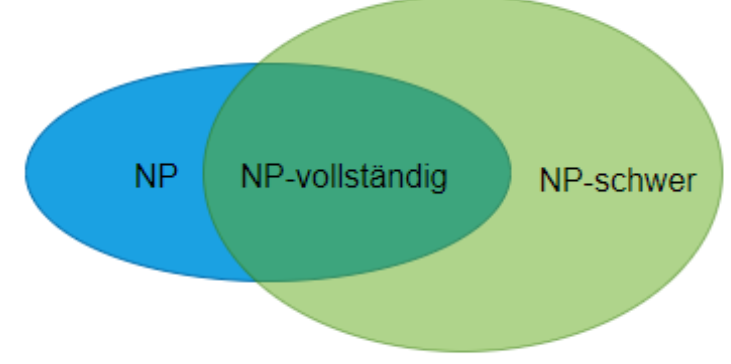
\includegraphics[width=0.5\linewidth]{images/p_vs_np.png}
\end{KR}

\begin{concept}{NP-schwer}\\
    Eine Sprache $L$ heisst $N P$-schwer, falls für alle Sprachen
    $$
    L^{\prime} \in N P \text { gilt, dass } L^{\prime} \preccurlyeq_{p} L
    $$
    Eine Sprache $L$ heisst NP-vollständig, falls $L \in N P$ und $L$ ist NP-schwer.
\end{concept}

\begin{definition}{Verifikation}\\
    Polynomzeit-Verifizierer: Überprüft die einzelnen Eingaben in einem Problem\\
    Zeuge: Informationen einer gültigen Eingabe
\end{definition}

\begin{KR}{Asymptotische Komplexitätsmessung}
    $O$-Notation (Landau Symbole)
    \begin{itemize}
        \item $f \in O(g)$: Es existiert ein $n_{0} \in \mathbb{N}$ und ein $c \in \mathbb{N}$, so dass für alle $n \geq n_{0}$ gilt
        \begin{itemize}
            \item $f(n) \leq c \cdot g(n) f$ wächst asymptotisch nicht schneller als $g$
        \end{itemize}
        \item $f \in \Omega(g)$: Es existiert ein $n_{0} \in \mathbb{N}$ und ein $d \in \mathbb{N}$, so dass für alle $n \geq n_{0}$ gilt
        \begin{itemize}
            \item $f(n) \geq \frac{1}{d} \cdot g(n) f$ wächst asymptotisch mindestens so schnell wie $g$
        \end{itemize}
        \item $f \in \Theta(g)$: Es gilt $f(n) \in O(g(n))$ und $f(n) \in \Omega(g(n))$
        \begin{itemize}
            \item $f$ und $g$ sind asymptotisch gleich
        \end{itemize}
    \end{itemize}
\end{KR}

\begin{concept}{Schranken für die Zeitkomplexität von U}
    \begin{itemize}
    \item $O(f(n))$ ist eine obere Schranke, falls
    \end{itemize}

    Eine TM existiert, die $U$ löst und eine Zeitkomplexität in $O(f(n))$ hat.

    \begin{itemize}
    \item $\Omega(g(n))$ ist eine untere Schranke, falls
    \end{itemize}

    Für alle TM $M$, die $U$ lösen, gilt dass $\operatorname{Time}_{\mathrm{M}}(n) \in \Omega(g(n))$
\end{concept}

\begin{formula}{Rechenregeln}
    \begin{itemize}
    \item Konstante Vorfaktoren $c$ ignorieren $(c \in O(1))$.
    \item Bei Polynomen ist nur die höchste Potenz entscheidend:
    \end{itemize}
    
    $$
    a_{k} n^{k}+a_{k-1} n^{k-1}+\cdots+a_{1} n+a_{0} \in O\left(n^{k}\right)
    $$
    
    \begin{itemize}
    \item Die $O$-Notation ist transitiv.
    \item $f(n) \in O(g(n)) \wedge g(n) \in O(h(n)) \rightarrow f(n) \in O(h(n))$
    \end{itemize}
\end{formula}

\begin{example}
    \begin{itemize}
        \item $O(n) \quad 7 n+4$
        \item $O(n^{3}) \quad 25 n^{2}+n^{3}+100 n$
        \item $O(n^{2} \cdot \log (n)) \quad n^{2}+n \cdot n \cdot(\log (n))+20 n^{2}+50 n \cdot 100$
        \item $O(2^{n}) \quad 10^{20}+3 n^{3}+2^{n}+2^{10} \cdot 2^{30}$
      \end{itemize}
\end{example}

\begin{KR}{Übersicht wichtigste Laufzeiten}
    \textbf{TODO:} Tabelle mit Laufzeiten
\end{KR}

\subsubsection*{Übersicht}
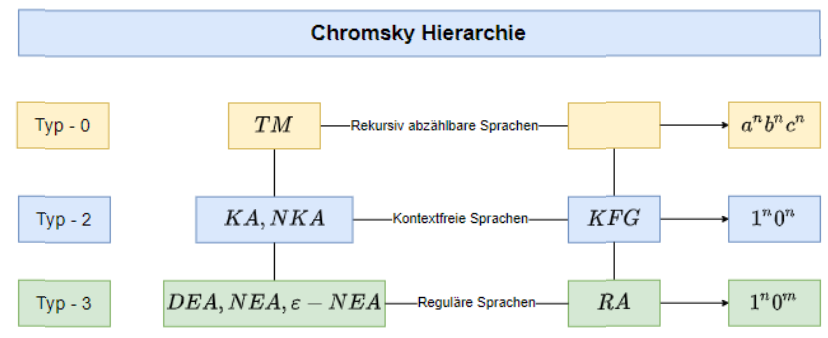
\includegraphics[width=0.8\linewidth]{images/chomsky_hierarchie.png}\\
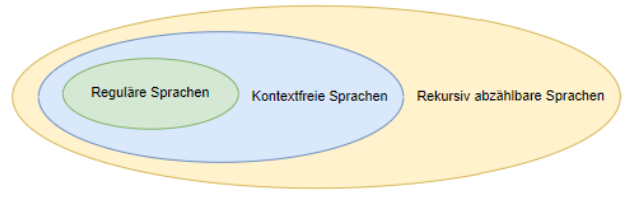
\includegraphics[width=0.5\linewidth]{images/sprachen.png}\\
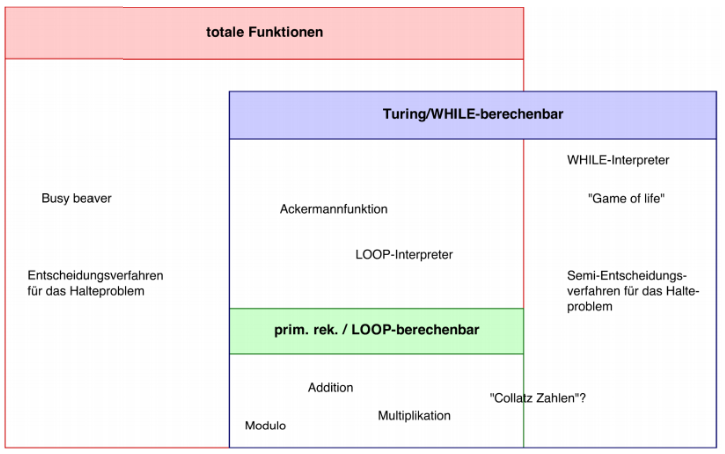
\includegraphics[width=1\linewidth]{images/funktionen.png}
